\documentclass[a4paper]{ctexart}
\usepackage[utf8]{inputenc}
\usepackage[a4paper]{geometry}
\usepackage{graphicx}
\usepackage{float}
\usepackage{hyperref}
\usepackage[heading = false]{ctex}
\usepackage{xcolor}
\usepackage{fontspec}
\usepackage{listings}
\pagestyle{plain}
\geometry{top=1.0cm, bottom=2.0cm}
\lstset{
    basicstyle = \ttfamily,
    commentstyle = \itshape,
    numbers = left,
    numberstyle = \zihao{-5}\ttfamily,
    frame = lrtb
}

\begin{document}
  \begin{titlepage}
      \songti
      \begin{center}
        \vspace*{2cm}
        
\includegraphics[width=0.7\textwidth]{../HDU.png}\\
        \vspace*{1cm}
        {\fontsize{36pt}{0}
          \textbf{机器学习实验\\报\quad 告\\}
        }
        \vspace*{12cm}
        {\fontsize{18pt}{0}
          \makebox[80pt]{\textbf{实验名称}} \underline{\makebox[250pt]{\Large 监督学习之多项式回归}}\\
          \vspace*{0.5cm}
          \makebox[80pt]{\textbf{学\qquad 院}} \underline{\makebox[250pt]{\Large 通信工程学院}}\\
          \vspace*{0.5cm}
          \makebox[80pt]{\textbf{专\qquad 业}} \underline{\makebox[250pt]{\Large xxxx}}\\
          \vspace*{0.5cm}
          \makebox[80pt]{\textbf{学\qquad 号}} \underline{\makebox[250pt]{\Large xxxx}}\\
          \vspace*{0.5cm}
          \makebox[80pt]{\textbf{学生姓名}} \underline{\makebox[250pt]{\Large xxx}}\\
        }
      \end{center}
  \end{titlepage}

  \CTEXsetup[format={\Large\bfseries}]{section}

  \newpage
  \section{实验目的}
  使用机器学习方法对面积和房价进行多项式回归拟合

  \section{实验内容与要求}
  \begin{itemize}
    \item 使用python sklearn包对房价数据建立多项式回归模型并进行训练
    \item 对结果进行可视化
  \end{itemize}

  \section{实验程序与结果}
  \subsection{程序代码}
  \lstinputlisting[language=Python]{lab2.py}
  \subsection{运行结果}
  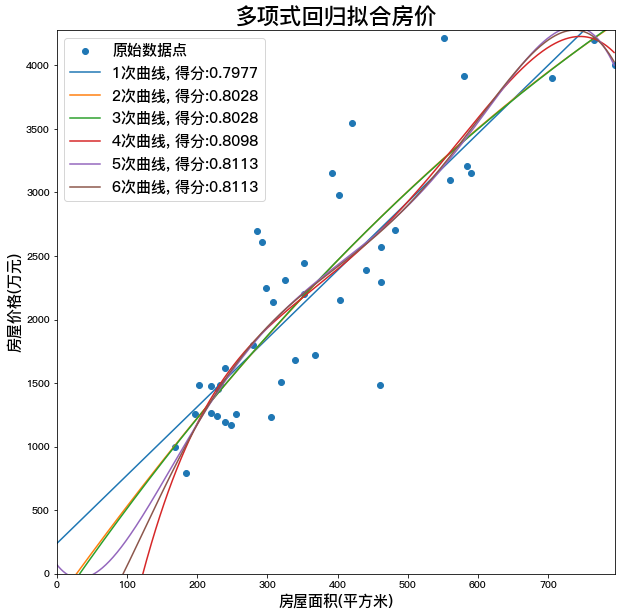
\includegraphics[width=1.0\textwidth]{fig/output.png}

  \section{实验结果分析}
  线性回归和非线性回归的区别,如在只有一个特征$x$时,线性回归只对一次参数做拟合,拟合多项式为$\hat{y}=b+wx$

  非线性回归对参数的一次项和高次项做线性回归,拟合多项式为$\hat{y}=b+w_1x+w_2x^2+w_3x^3+...$

  从得分可以看出,最高次项的次数越高,得分越高,即误差越小;但次数越高,曲线越不符合实际情况

\end{document}
